\subsection{Problem Formulation}
\label{sec:problem}

%\subsection{Geolocated Time Series}
%\label{subsec:geoTS}

A {\em time series} is a time-ordered sequence of values $T = \{v_1, \ldots, v_n\}$, where $v_i$ is the value at the $i$-th time point and $n$ is the length of the series. In this work, we specifically deal with {\em geolocated time series}~\cite{chatzig17btsr}, i.e., time series that are additionally characterized by a \emph{location}, denoted by $T.loc$. Assuming a 2-dimensional space, we further use the notation $T.loc_x$, $T.loc_y$ to refer to the $(x,y)$ coordinates of $T$'s location. In the rest of the paper, when it is clear from the context, we also refer to such geolocated time series as {\em objects} for brevity.

%The following distance measures are used, either in building, or when traversing the indices to generate the geolocated time series summaries.

To quantify the proximity of two geolocated time series in the {\em spatial domain}, we measure the distance of their respective locations. More specifically:

\begin{mydefinition}[Spatial Distance]
The {\em spatial distance} between two geolocated time series $T$ and $T'$ is calculated using the Euclidean distance of their respective locations. Furthermore, we normalize this distance with $maxDist_{sp}$, i.e., the maximum spatial distance of any pair of objects in the dataset, to obtain a measure in the interval $[0,1]$. Thus:
\begin{equation} \label{eq:dist_sp}
dist_{sp}(T, T') = \frac{\sqrt{(T.loc_x - T'.loc_x)^2 + (T.loc_y - T'.loc_y)^2}}{maxDist_{sp}}. 
\end{equation} \label{eq:2}
\qed
\end{mydefinition}

Moreover, we measure similarity in the {\em time series domain}. Similarly to other prior works (e.g., \cite{shieh2008kdd}), we apply the Euclidean distance in this domain. In future work, we plan to make use of more complex distance measures \cite{paparrizos2015k}.
More specifically:

\begin{mydefinition}[Time Series Distance] The {\em time series distance} between two time series $T$ and $T'$ of equal length $n$ is calculated as:
\begin{equation} \label{eq:dist_ts}
dist_{ts}(T, T') = \frac{\sqrt{\displaystyle \sum_{i=1}^{n}(T.v_i - T'.v_i)^2}}{maxDist_{ts}}
\end{equation}
\noindent where $maxDist_{ts}$ denotes the maximum distance on the time series domain of any pair of objects in the dataset and is used for normalization, as above. \qed
\end{mydefinition}


%\subsection{Summary Formulation}
%\label{subsec:summaries}

Our objective in this paper is to compactly represent a large number of geolocated time series by some form of summaries so as to support and facilitate their visual exploration. Intuitively, given a set of geolocated time series, we want to provide summaries that express both their pattern across time as well as their corresponding spatial extent. These summaries may be constructed over the whole dataset, e.g., to provide an initial quick overview of the whole data, or over the results of a previous query, e.g., over those time series located inside a bounding box drawn by the user on the map. Specifically, we consider two types of summaries, called \emph{bundle summaries} and \emph{tile map summaries}, respectively, which we describe next.

%, which consist of the following two summarization methods intended for visual exploration of geolocated time series.

%\checknote{Instead of calling them ``summaries'', should be called aggregates? After all, it is clear from the definition that each one is derived after a query with specific parameters is executed against the index.}

\subsubsection{Bundle Summaries}
\label{subsec:bundle_sums}

%The user may also specify a spatial area $q$ of interest, filtering out objects having locations outside this area.

%\vspace{10pt}
%
%\noindent \emph{Bundle Summaries}. 

This type of summary is composed of a set of $k$ {\em ``bundles''}, where each bundle comprises the following information:

\begin{itemize}
\item a cluster of similar time series in the temporal domain
\item a set of Minimum Bounding Rectangles (MBRs) summarizing in the spatial domain the respective locations of those time series
\item an integer indicating the number of objects located within each of the above MBRs.
\end{itemize}

To derive such bundles, we use the notion of {\em Minimum Bounding Time Series} (MBTS) introduced in \cite{chatzig17btsr}. An MBTS bundles together a set of time series  $\mathcal{T}$ using a pair of bounds that fully contain all of them.  Figure~\ref{fig:example_bundle} depicts an example of two MBTSs for two disjoint sets of time series. Formally:

\begin{mydefinition} [Minimum Bounding Time Series (MBTS)]
Given a set of time series $\mathcal{T}$, its MBTS consists of an \emph{upper bounding time series} $T^{\sqcap}$ and a \emph{lower bounding time series} $T^{\sqcup}$, constructed by respectively selecting the maximum and minimum of values at each time point among all time series in set $\mathcal{T}$ as follows:
\begin{align}\label{eq:bounds1}
 \begin{split}
  & T^{\sqcap} = \{ \max_{T \in \mathcal{T}} T.v_1, \ldots, \max_{T \in \mathcal{T}} T.v_{n} \} \\
  & T^{\sqcup} = \{ \min_{T \in \mathcal{T}} T.v_1, \ldots, \min_{T \in \mathcal{T}} T.v_{n} \}.
 \end{split}
\end{align}
\qed
\end{mydefinition}


\begin{figure}[t]
	\centering
	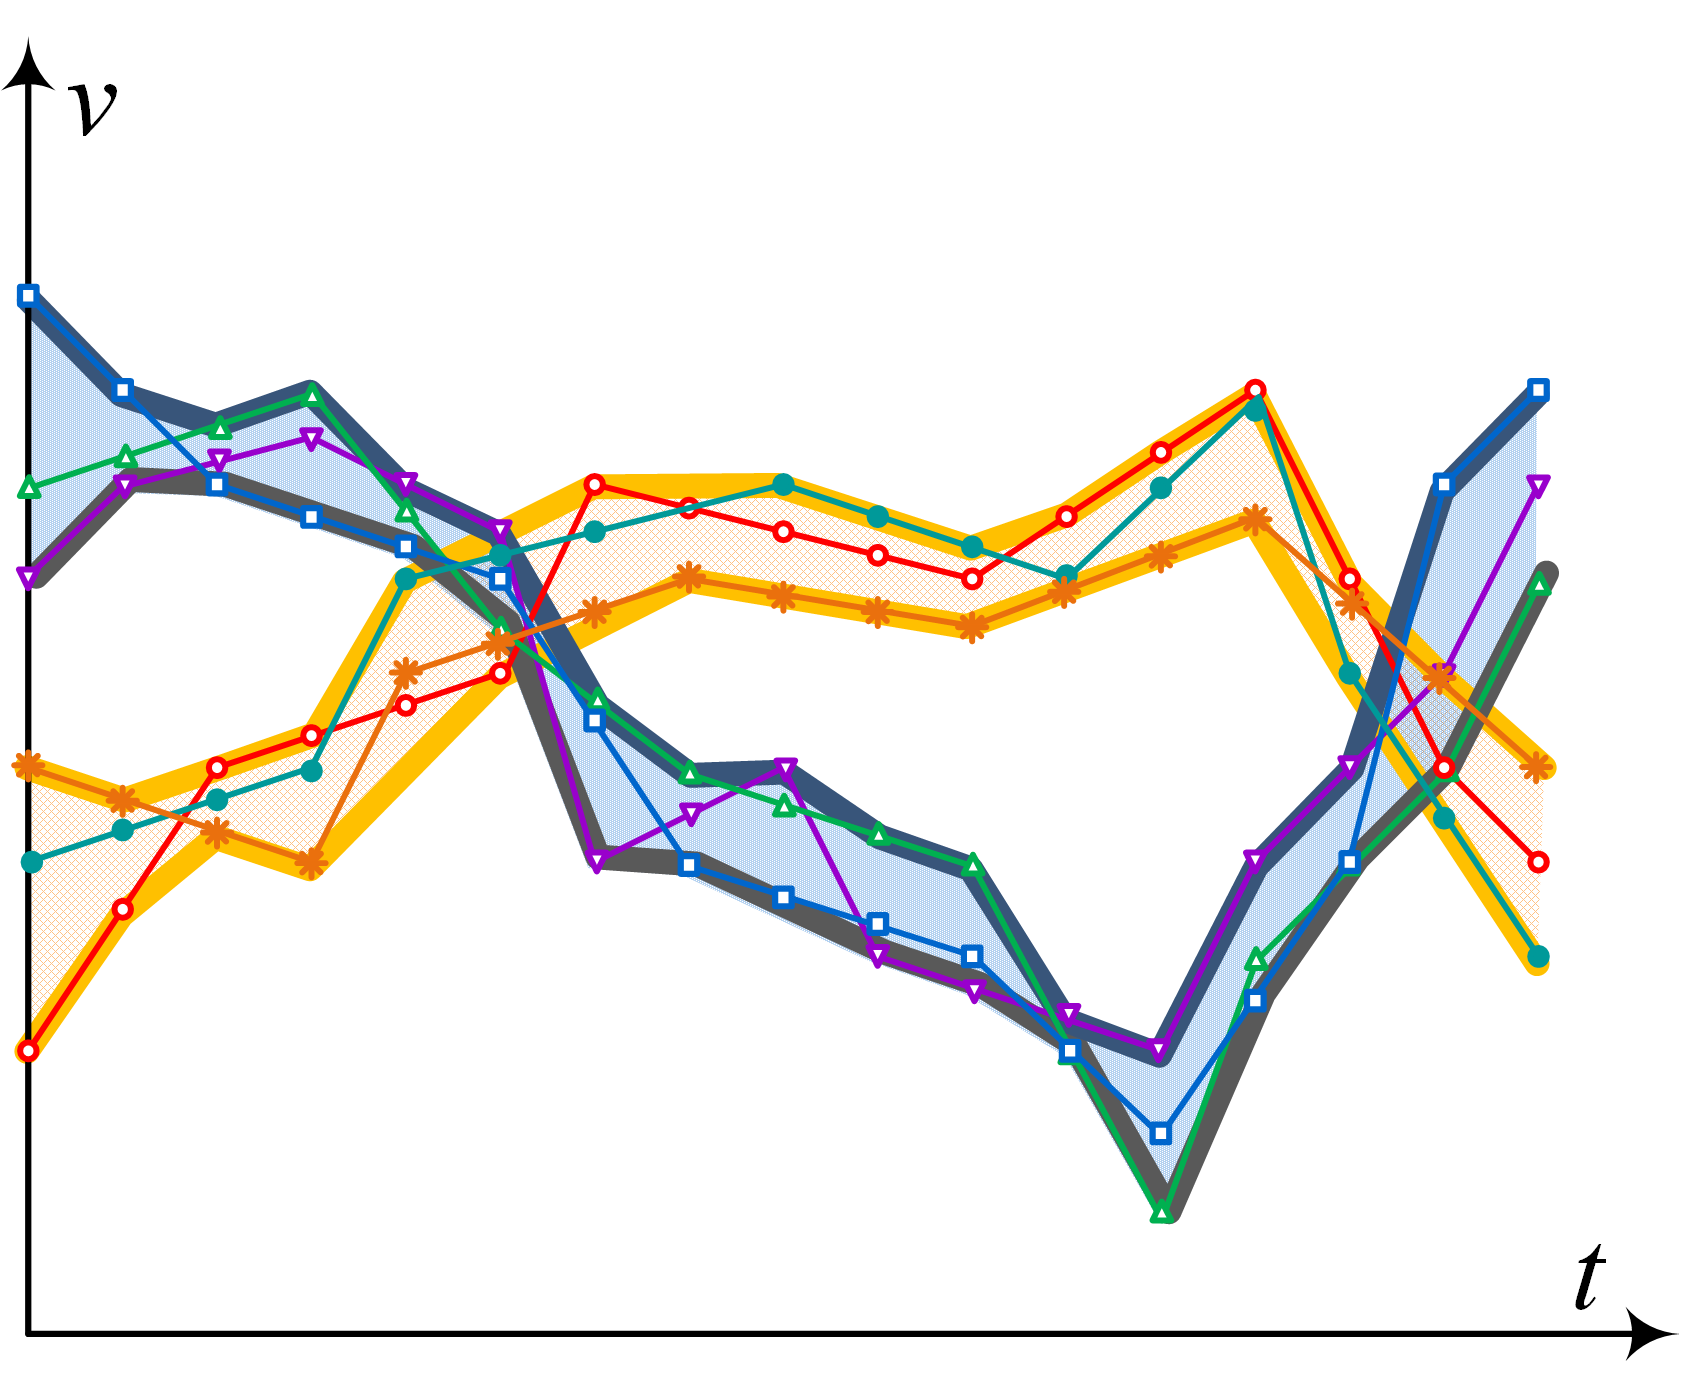
\includegraphics[width=0.5\textwidth]{figures/bounds_btsr.png}
	\vspace{-7.5pt}
	\caption{Example illustrating the resulting bundles for two sets of time series.}
	\vspace{-7.5pt}
	\label{fig:example_bundle}
\end{figure}


%The bundles provide a summarization of the time series that are contained within their MBTSs. Figure~\ref{fig:example_bundle} depicts an example of two time series bundles for two different sets of time series. Regarding the spatial summary, for each MBR associated with a certain bundle, the counter denotes the number of time series contained in it.


%Hence, a bundle summary can be defined as follows:

Hence, we can formulate the problem of summarizing a set of geolocated time series by means of a bundle summary as follows:

\begin{problem} [Bundle Summary]
Given a set $\mathcal{T}$ of geolocated time series, a spatial area $q$ of interest, a number $k$ of desired bundles, and a number of $l$ MBRs per bundle, the problem is to efficiently compute a {\em bundle summary} that consists of a list of $k$ tuples over the subset $\{ T \in \mathcal{T} : within(T.loc, q) \}$ of time series located within area $q$. Each such tuple in the bundle summary has the following structure:
\begin{equation} \label{eq:bundles_sum}
R_b = \{ \langle mbts, \{\langle mbr, cnt \rangle \}\rangle\}
\end{equation}
\noindent where $mbts$ is a time series summary in the form of MBTS and is associated with a list of $l$ MBRs; the count $cnt$ of objects within each such $mbr$ is also available.
\qed
\end{problem}

In Section~\ref{sec:bundles_summary}, we show how the \btsr index can be used to address this problem, i.e., to efficiently compute bundle summaries.


\subsubsection{Tile Map Summaries} 
\label{subsec:tilemap_sums}

%\vspace{10pt}
%
%\noindent \emph{Tile Map Summaries}. 

The bundles in the summary type introduced above are formed in a {\em data-driven} manner, as objects belonging to the same bundle should be similar (e.g., based on clustering). An alternative way to visually highlight spatio-temporal patterns in a large set of geolocated time series is through summaries that rely on a {\em fixed partitioning} of the time series domain. More specifically, the entire domain may be subdivided into adjacent, non-overlapping {\em tiles} (Figure~\ref{subfig:tile_map}), so that each tile captures the portion of a time series falling within this tile. Simple aggregates (e.g., counts) of time series per tile can easily convey the distribution of values in the dataset. As shown in the example, the higher the concentration of data points within a tile, the darker its shade. More formally:


\begin{mydefinition} [Tile Map]
Let the {\em time domain} $[t_{min}, t_{max})$ be divided into successive intervals of equal size $\tau$, resulting into a subdivision $\{[t_{min}, t_{min}+\tau), [t_{min}+\tau, t_{min}+2\tau), \dots, [t_{max}-\tau, t_{max})\}$. Subdivision of the {\em value domain} $[v_{min}, v_{max})$ is carried out using a finite number of {\em breakpoints} $\{v_1, v_2, \dots, v_h\}$ where $v_1 = v_{min}$, and $v_h = v_{max}$, wheareas the rest may be arbitrary values provided that $v_1 < v_2 < \dots < v_h$. This subdivision yields disjoint, consecutive segments $\{[v_{min}, v_1), [v_2, v_3), \dots, [v_h, v_{max})\}$ in the value axis. The resulting {\em tile map} is a matrix of tiles over both domains, so that tile $(i,j)$ corresponds to time interval $[t_{min}+i\cdot\tau, t_{min}+(i+1)\cdot\tau)$, $i \in {0,\dots,\ceil*{\frac{t_{max}-t_{min}}{\tau}}}$, and to value segment $[v_j, v_{j+1})$, $j \in {0, \dots, h-1}$.
\end{mydefinition}

Essentially, such a tile map has a similar effect as {\em space-driven} partitionings like quadtrees or grid subdivisions \cite{2001:SDA:377296}. As in the case of spatial objects, a time series can be checked for containment within each tile. More specifically, a time series data point $v_t$ at time $t$ is contained in tile $(i, j)$ if $t_{min}+i\cdot\tau \leq t < t_{min}+(i+1)\cdot\tau$ and $v_j \leq v_t < v_{j+1}$. Once all time series are mapped into tiles, this matrix offers a summary of the entire dataset.

However, we may inspect specific portions of a tile map, by checking a group of neighboring tiles. This can be abstracted as a {\em timebox}~\cite{hochheiser2003interactive} applied over both domains. Intuitively, such a timebox is a rectangle in the time series domain that fully contains a set of time series in the time and value range that it represents. Figure~\ref{subfig:timebox} depicts with green color the time series that are contained within a timebox, among a set of time series. More specifically:


\begin{mydefinition} [Timebox]
A {\em timebox} $p$ specifies a time interval $[t,t')$ and a value range $[v,v')$ in order to identify any qualifying time series. We denote as $timebox(T, p)$ once a time series $T$ qualifies to this timebox $p$ if $\forall t_i \in [t,t'), v \leq T.v_i < v'$.  
\end{mydefinition}

Overall, given a timebox $p$ and a spatial area $q$ of interest over a set of geolocated time series, we are interested in identifying:
\begin{itemize} 
\item The tiles that summarize objects located within $q$ and are also fully included within $p$, i.e., no data point of the time series falls outside $p$ in the respective time interval.
\item In addition, the summary provides also a set of $k$ MBRs covering all qualifying time series; a counter measures the time series contained within each such MBR. 
\end{itemize}
 
%More formally, such a {\em tile map summary} can be defined as follows:
We can now formulate the problem of computing {\em tile map summaries} as follows:


\begin{problem} [Tile Map Summary]
Given a set $\mathcal{T}$ of geolocated time series, a timebox $p$ and a spatial area $q$ of interest, and a number $k$ of desired MBRs, a {\em tile map summary} provides a list of $k$ tuples over the subset $\{ T \in \mathcal{T} : within(T.loc, q) \wedge timebox(T, p) \}$ of time series located within area $q$ and qualifying to timebox $p$. Each such tuple in the tile map summary has the following structure:

\begin{equation} \label{eq:tmap_sum}
R_t = \{ \langle tmap, \{\langle mbr, cnt \rangle \}\rangle\}
\end{equation}

\noindent where $tmap$ represents the tile map constructed over the qualifying time series and is associated with a list of $k$ MBRs that outline their spatial extent; the count $cnt$ of objects within each such $mbr$ is also available.
\qed
\end{problem}


In Section~\ref{sec:tilemap_summary}, we propose a technique that can efficiently construct tile map summaries by employing an extended variant of the \isax index.